\section{Experimental setup}
Like mentioned at the beginning the main goal of this experiment is to measure the absorption spectrum of rubidium.
In the following we will present the experimental setup that allows at the end to measure the intensity of a laser beam
behind a gas cell as a function of frequency. The single steps of calibration and experimental results will be discussed
in the next section.

The length $L$ of the external cavity can be varied with a piezo modulator. The expansion of piezo crystals can be manipulated by an
applyed voltage. Using a triangular voltage signal we can execute a periodic variation of $L$ and thus a sweep in laser frequeny. The
modulation can be applied to the piezo or simultaniously to the diode current.

The overall setup is displayed in figure~\ref{fig: setup}.

\begin{figure}
\centering
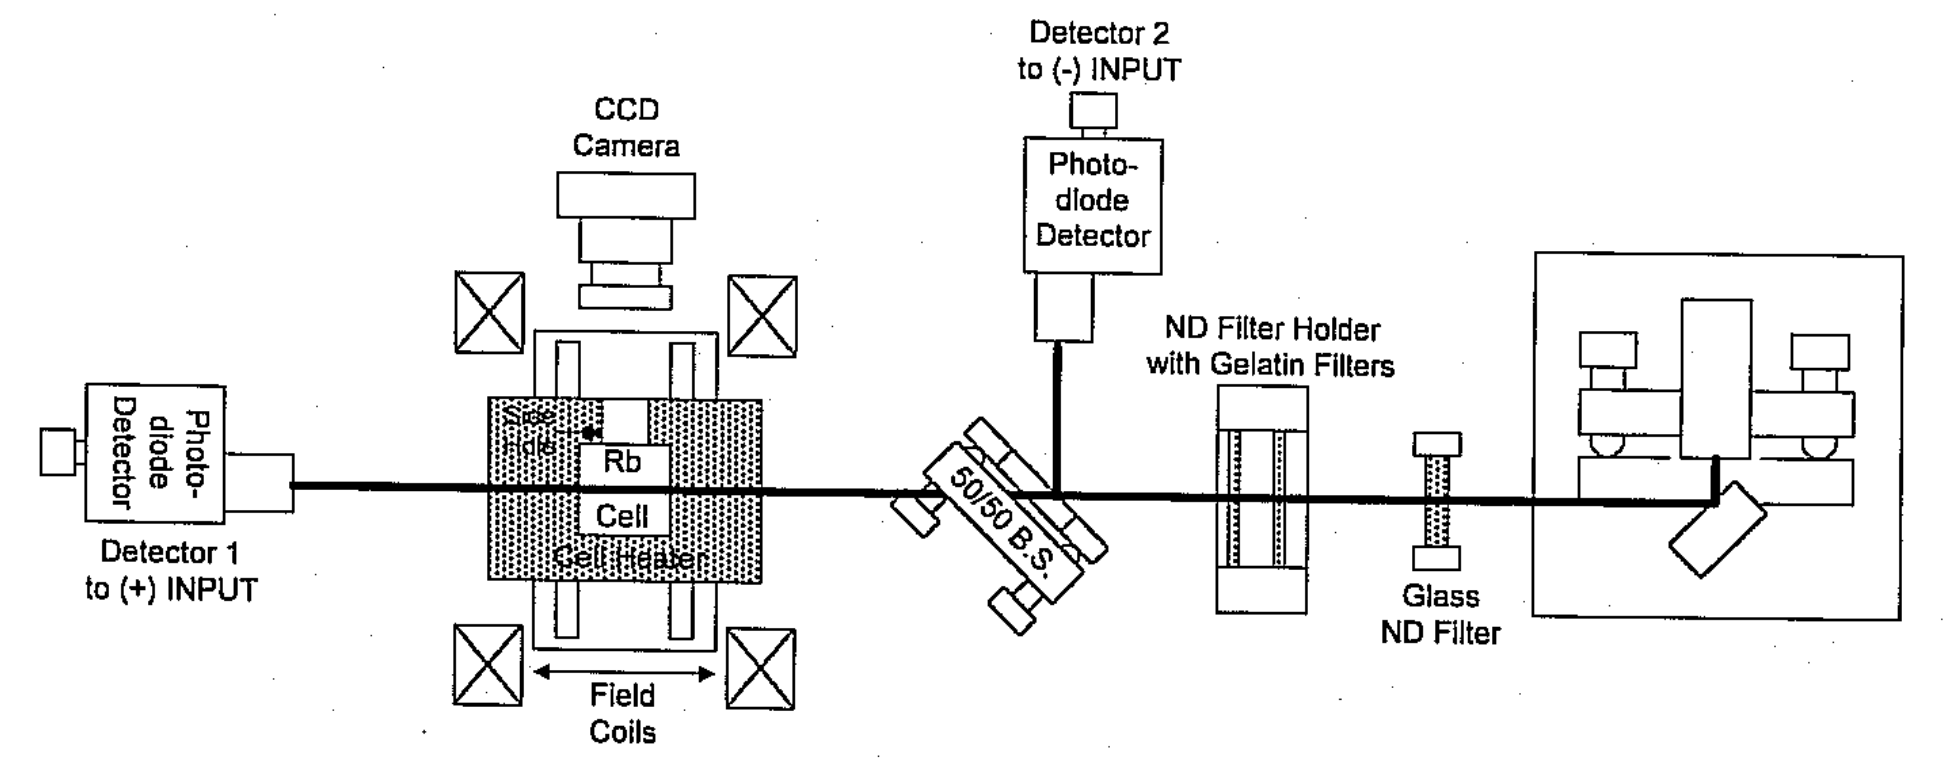
\includegraphics[width = \textwidth]{pics/setup.png}
\caption{Experimental setup for measuring the absorption spectrum of gaseous rubidium. Threw the calibration 
process not all components are used in each step (see section~\ref{} for details) \cite{anleitung60}. }
\label{fig: setup}
\end{figure}


The laser intensity is measured with photodiodes since the photo current
is propotional to the incoming light intensity.
